\subsection{Fermi-Verteilung}
Fermi-Verteilung ist Ergebnis eines dynamischen Gleichgewichts bei einer Temperatur
\subsection{Fermi-Niveau im Nichtgleichgewicht}
	
	\subsection{Generation und Rekombination}
		Generation ist Erzeugung von Ladungsträgern (eines Elektrons und eines Lochs) unter Energiezufuhr (Wärme, Strahlung usw.).
		\newline
		
		Rekombination ist der Übergangsprozess von einem Elektron aus dem Leitungsband-Zustand in einen Valenzband-Zustand. Unter Energieabgabe werden so Ladungsträger
		(Elektronen und Löcher) vernichtet.
		\newline
		
		Bei diesen Prozessen bleibt die Gesamtladung erhalten.
		\newline
		
		Im thermischen Gleichgewicht sind G und R gleich groß
		\newline
		
	\subsubsection{Überschuss-Ladungsträger}
	
	Überschuss-Ladungsträger ergibt sich aus dem Delta der Anzahl der freien Elektronen n und der Freien Elektronen bei Eigenleitung $n_0$
	\newline
	$\Delta n=n - n_0$
	
	\subsection{Lebensdauer}
	Ladungsträgerlebensdauer ergibt sich aus dem Quotient aus Überschuss-Ladungsträgern $\Delta n$ und Rekombinationsrate R
	\newline
	
	$\tau =\frac{\Delta n}{R}$
	
	
	\subsubsection{Rekombinationsrate}

	Die Rekombinationsrate R ist der Quotient aus Überschussladungsträgern und der Ladungsträgerlebensdauer $\tau$
 
		$R =\frac{\Delta n}{\tau}$
		\newline
		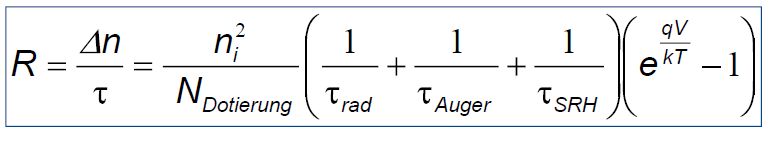
\includegraphics[width=0.4\linewidth]{Kapitel/Kap05/Rekombinationsrate}
		

	
	\subsubsection{Verschiedene Rekombinationsmechanismen}
	Es gibt verschiedene Rekombinationsmechanismen.
	\begin{enumerate}
		\item Strahlende Rekombination:
			\newline
			Elektron springt durch Energieabgabe durch Aussenden von Licht vom Leitungsband ins Valenzband. (Funtermentaler Prozess der direkten Halbleiter)
		\item Auger-Rekombination:
			\newline
			Auger-Rekombination ist ein sog. strahlungsloser Übergang. Sie benötigt drei Ladungsträger. Dabei wird die Energiedifferenz, die ein Elektron vom Sprung von Leitungs- in das Valenzband abgibt auf ein anderes Elektron übertragen, welches auf ein höheres Energieniveau gehoben wird. 
			\newline
			Mit zunehmender Ladungsträgerkonzentration (z.B. bei starker Dotierung) erhöht sich die Rekombinationsrate
		\item Defekt-Rekombination (Shockley-Read-Hall):
			\newline
			Die Defekt-Rekombination ist ein zwei-Stufen-Prozess, bei dem ein Elektron über einen Defektzustand/Störstelle (z.B. eine Verunreinigung durch andere Metalle) vom Leitungsband in das Valenzband spring. Die Energiedifferenz wird durch Aussendung von Licht bewirkt.
			\newline
			Es handelt sich um den Hauptverlustmechanismus in Silizium-basierten Bauelementen (Verringerung von Ladunsträgerlebensdauer). Die (geringe) Defektdichte (z.B. Verunreinigung, Kristallfehlordnung) ist daher das Maß für die Materialqualität.
		\item Oberflächen-Rekombination:
			\newline
			An Oberflächen des Halbleiters existieren lokalisierte Zustände,
			die sich nicht in die Bandstruktur einfügen. Die Rekombination findet wie bei der SRH statt.
			Oberflächenrekombination kann nur in Kombination mit Ladungsträgertransport zur Oberfläche geschehen.
			Rekombination am Metallkontakt läuft über die kontinuierliche
			Zustandsverteilung des Metalles ab und wird nür über den Transport der Ladungsträger im Halbleiter limitiert.
	\end{enumerate}



\begin{center}
	
	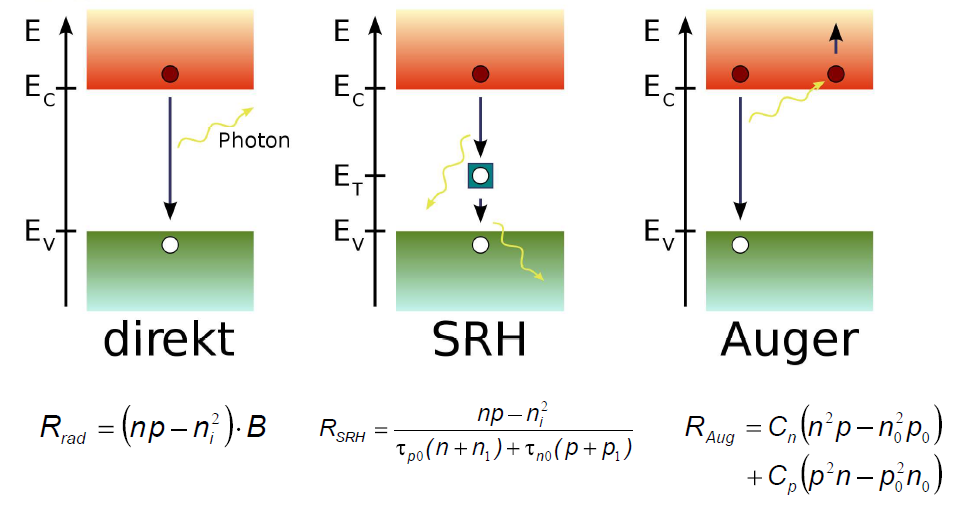
\includegraphics[width=0.7\linewidth]{Kapitel/Kap05/Rekombinationsarten1.png}
	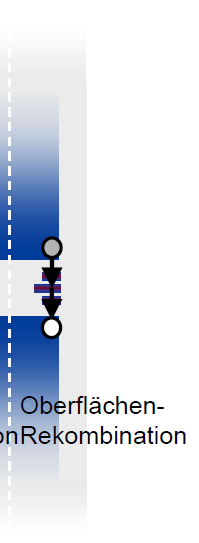
\includegraphics[width=0.15\linewidth]{Kapitel/Kap05/Rekombinationsarten2}
\end{center}

	
\subsection{Ortsabhängiges Energiebanddiagramm}
	Betrachtet man Halbleiter so ist zu Erkennen, dass die Energiebänder verbogen und damit Ortsabhängig sind.

\begin{center}
	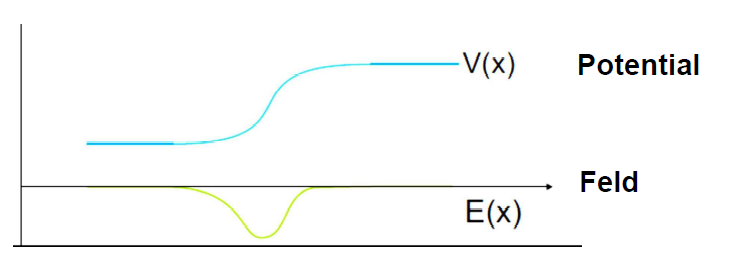
\includegraphics[width=0.5\linewidth]{Kapitel/Kap05/Ortsabhaengiges_Energiebanddiagramm.png}
	$E(x) = \frac{\delta V(x)}{\delta x}$
\end{center}





\subsection{Poisson-Gleichung}
Mit Hilfe der Poisson-Gleichung ist es möglich, die Bandverbiegung mit den Ladungsverteilungen im Inneren des HL in Verbindung zu bringen.

\begin{center}
	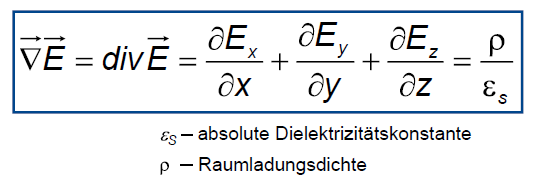
\includegraphics[width=0.5\linewidth]{Kapitel/Kap05/Poissongleichung}
\end{center}
Die hier als Poisson-Gleichung bezeichnete Maxwell'sche Gleichung, stellt einen allgemein gültigen Zusammenhang zwischen der Raumladungsdichte und dem Elektrischen Feld dar.

\subsubsection{Gradienten und Ströme}
Wenn Fermi-Level als "Füllstand" angesehen werden kann, dann erzeugt ein Gradient des Füllstandes einen Strom:

\begin{center}
	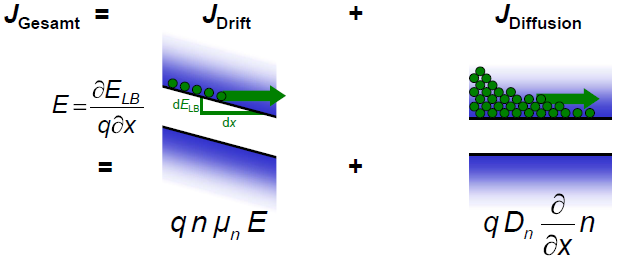
\includegraphics[width=0.7\linewidth]{Kapitel/Kap05/Gradient}
\end{center}
Gradient des Fermi-Levels gibt Netto-Stromrichtung an
\begin{center}
	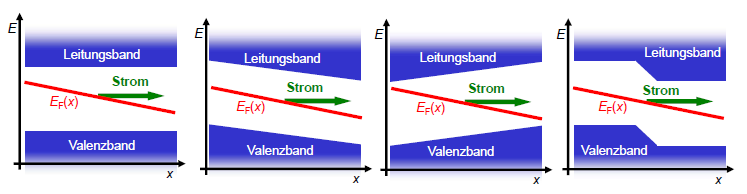
\includegraphics[width=0.6\linewidth]{Kapitel/Kap05/FerminiveauverlaufBeispiele}
\end{center}
Wenn der Verlauf des Fermi-Levels bekannt ist, d.h. der Gradient des Fermilevels, so ist die Richtung des Stromes gegeben, unabhängig von Bandkanten- (Feld-) Verlauf!

\subsection{Kontinuitätsgleichung}
Die Kontinuitätsgleichung vereint  Transport-, Rekombinations- und Generationsmechanismen in einer Gleichung, auf Basis der Ladungsträgererhaltung

\begin{center}
	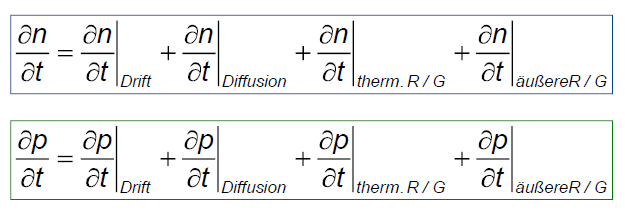
\includegraphics[width=0.7\linewidth]{Kapitel/Kap05/Kontinuitaetsgleichung}
\end{center}

Der Gesamtstrom hängt linear ab von:
\begin{itemize}
	\item der Beweglichkeit der Ladungsträger
	\item der Feldstärke (angelegten Spannung)
	\item dem Gradienten der Ladungsträgerkonzentration
\end{itemize}

\subsection{Minoritätsladungsträger-Diffusion}
	Zu viele Details --> vermutlich nicht relevant
	
	\subsubsection{Lösungen für Spezialfälle}
	Zu viele Details --> vermutlich nicht relevant
	
	
\subsection{Zwei Halbleiter im Kontakt}
	Kommen zwei Halbleiter in Kontakt hat man einen Halbleiterübergang, der aus verschiedenen oder verschieden dotierten Materialien besteht.
	Hierbei unterscheidet man zwischen:

	\begin{itemize}
		\item Homoübergang: Beide Halbleiter bestehen aus demselben Material 
		\item Heteroübergang: Beide Halbleiter bestehen aus verschiedenen Materialien und haben verschiedene Bandlücken		
	\end{itemize}
	Die Dotierung der beiden Materialen kann vom gleichen Typ oder entgegengesetzt sein (pn-Übergang)
	\subsubsection{Offsets, Typ I, II, III}
	Der Offset beschreibt den Übergang der Bandlücke (das Delta) zwischen den Leitungs- bzw. Valenzbändern der beiden Materialien. Bandoffsets können Barrieren sein.
	
	% offset graphik
	\begin{center}			
		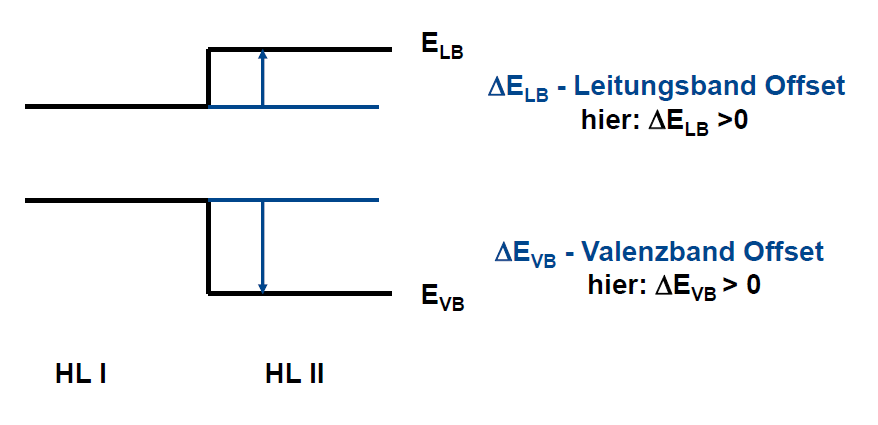
\includegraphics[width=0.7\linewidth]{Kapitel/Kap05/Offset.png}
	\end{center}
	
	Auf Basis des Offsets unterscheidet man zwischen drei Typen von Heteromaterialien:
	
	\begin{center}
	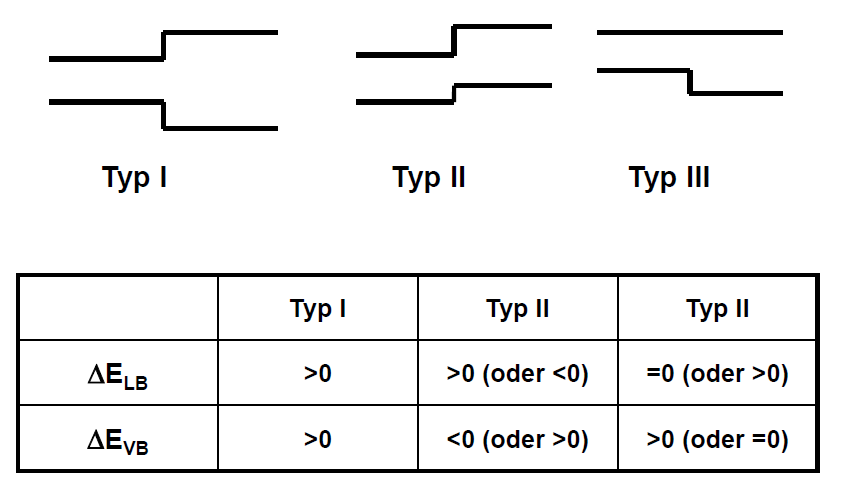
\includegraphics[width=0.7\linewidth]{Kapitel/Kap05/TypI-III}
	\end{center}
	
	\subsubsection{Injektion, Akkumulation, Extraktion, Exklusion}
	(Dieses Block wurde nicht in der Klausurenzusammenfassung der Übung erwähnt, der Vollständigkeitshalber wurde er mit aufgenommen)
	\newline
	Sind zwei Halbleiter in Kontakt gibt es unterschiedliche Beweglichkeiten und unterschiedliche Diffusion in beiden HLn.
	
	Hierbei gibt es Verschiedene Diffusions- und Driftströme
	Hierbei unterscheidet man 4 Arten
	\newline
		\begin{center}
			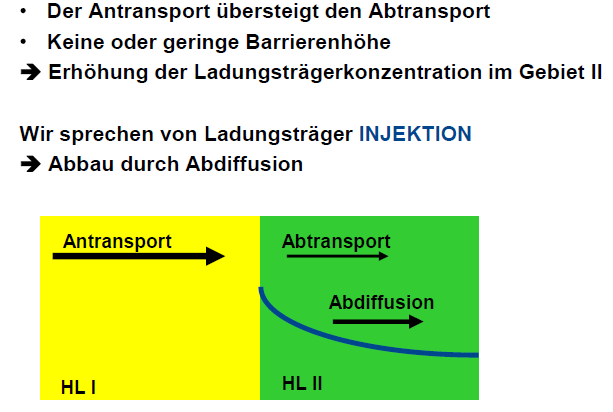
\includegraphics[width=0.45\linewidth]{Kapitel/Kap05/Interjektion}
			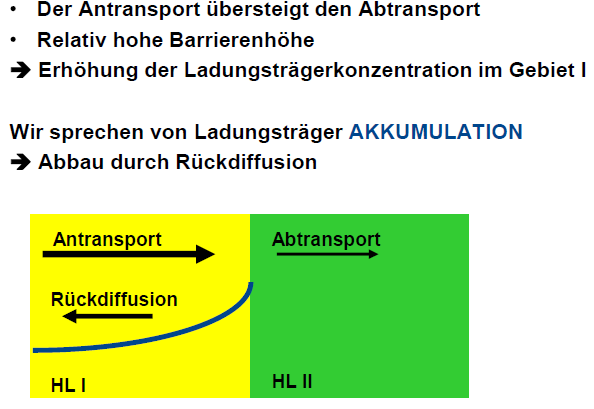
\includegraphics[width=0.45\linewidth]{Kapitel/Kap05/Akkumulation}
		\end{center}
	
		\begin{center}
			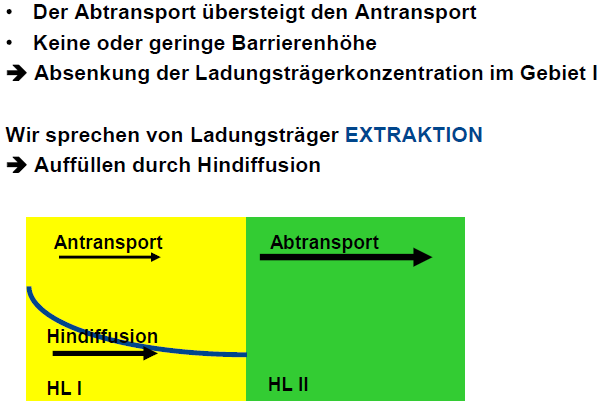
\includegraphics[width=0.45\linewidth]{Kapitel/Kap05/Extraktion}
			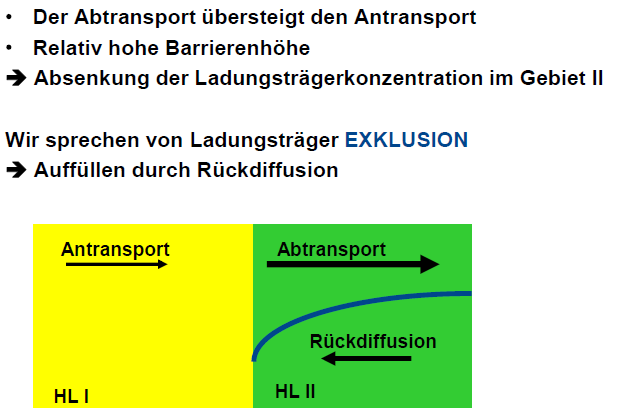
\includegraphics[width=0.45\linewidth]{Kapitel/Kap05/Exlusion}		
		\end{center}
			
\todo{Fragen aus Own Clowd zuordnen}
\todo{Gruppenübungs-Inhalte ergänzen}